
\section{Búsqueda de parámetros óptimos }

El principal objetivo de esta sección es encontrar los parámetros óptimos de knn y knn+pca con respecto a la accuracy. 

\subsection{Experimentación preliminar}
Este primer segmento de la sección se enfoca en generar una intuición sobre cómo reaccionan los métodos frente a distintos valores de k, alpha para ello utilizamos una partición del dataset original para poder experimentar sobre un rango bastante extenso de parámetros sin preocuparnos demasiado por la complejidad. Este primer experimento consiste en utilizar un split simple de train y validación sobre la partición previamente elegida para cada k en el caso de kNN y para cada pareja alpha, k en caso de kNN+PCA. 

\subsubsection{kNN}

\begin{figure}[h]
\begin{subfigure}{0.5\textwidth}
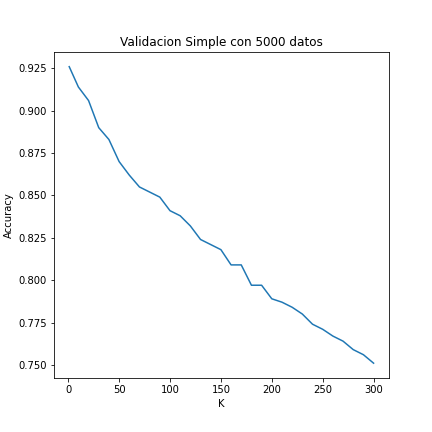
\includegraphics[width=0.9\linewidth, height=5cm]{images/validacionSimple_knnsolo.png} 
\caption{Rango de 1-300 con granularidad 10}
\label{fig:subimbar_medio1}
\end{subfigure}
\begin{subfigure}{0.5\textwidth}
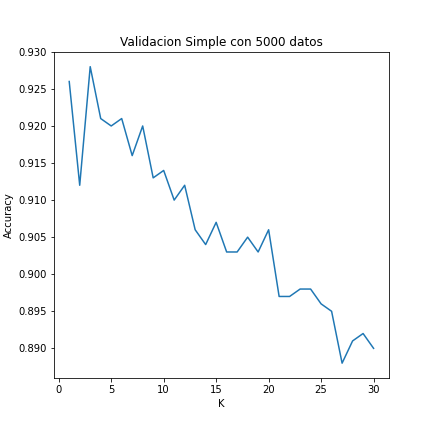
\includegraphics[width=0.9\linewidth, height=5cm]{images/validacionSimple_knnsolo_Kchicos.png} 
\caption{Rango de 1-30 con granularidad 1}
\label{fig:subimbar_medio2}
\end{subfigure}
\caption{Validación Simple de kNN sobre el dataset reducido.}
\label{knn_preliminar}%
\end{figure}

\par

Como podemos primer en la imagen (a) de Figura 1 muestra una presunta relación inversamente proporcional entre el k elegido y su accuracy, para vislumbrar si esto es así realizamos el mismo experimento sobre valores pequeños de k pero con más granularidad para notar cualquier variación en la accuracy, qué es lo que se puede observar en la imagen (b). Ahora con más detalle se puede observar a partir de cuales magnitudes el método disminuye se eficiencia, en particular los mejores k parecen encontrarse dentro del rango 1-10.

\subsubsection{kNN+PCA}

\begin{figure}[H]
    \centering
    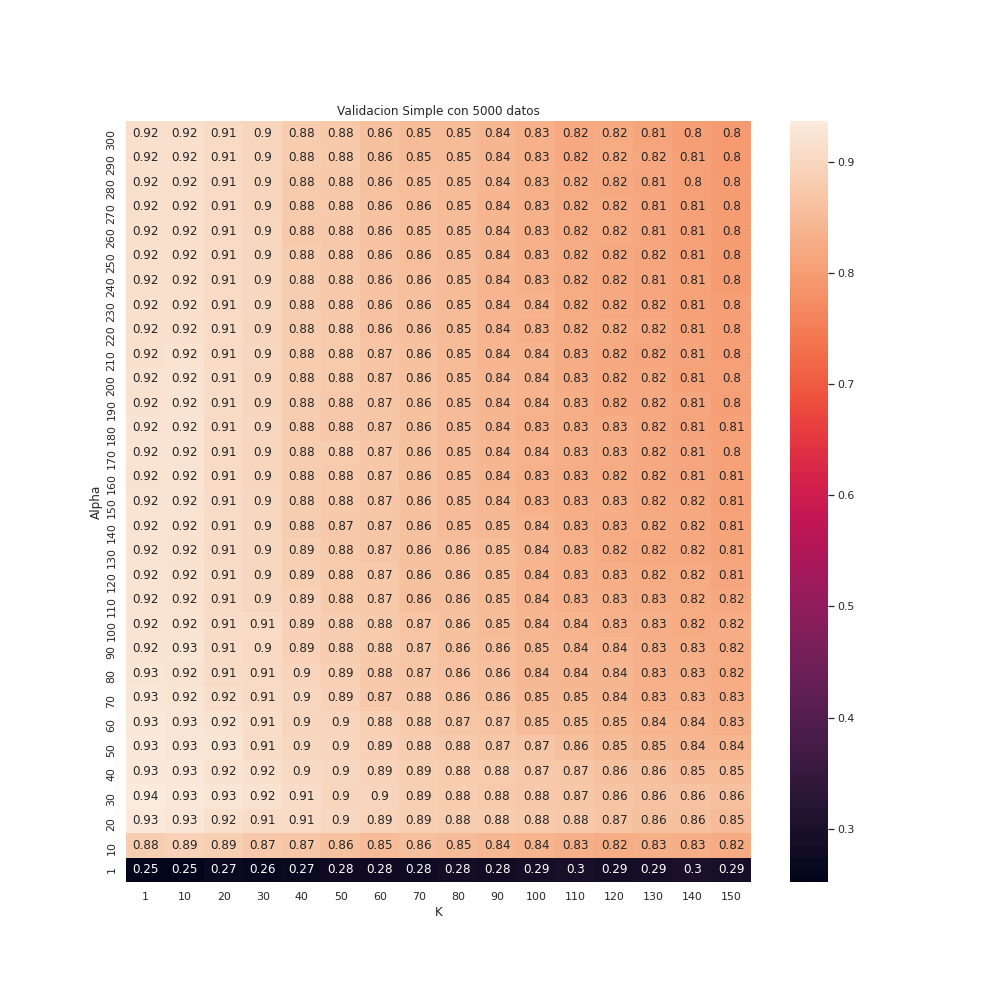
\includegraphics[width=12cm]{images/validacionSimple_heatmap_datasetRedux}%
    \qquad
    \caption{Validación Simple de kNN+PCA sobre el dataset reducido}
    \label{knnpca_preliminar}%
\end{figure}

Al igual que sucede en kNN podemos notar un mejor desempeño para las parejas con valores chicos de $k$, en cambio para alpha ya no está clara la relación aunque se puede ver una leve mejora para los $alpha$ menores a 100, por esto mismo en la validación simple que sigue sobre el dataset en su totalidad mantendremos el rango del $alpha$ y solo achicamos el de $k$.

\subsection{Validación Simple sobre el data-set completo}

La segunda parte de esta sección realiza el mismo experimento que la primera pero ahora sobre el dataset original y eligiendo un rango condicionado por lo antes visto, con la motivación de encontrar el conjunto de los mejores diez parámetros para cada método. Notese que cuando decimos que el rango del experimento estará condicionado por una experimentación realizada sobre un dataset reducido ,estamos asumiendo que los parámetros se ven inmutables por la cantidad de datos para entrenar y validar lo cual no es trivial por esa razón lo analizamos en la SECCIÓN FER, donde mostramos empíricamente que esto es verdadero para nuestro caso particular.


\subsubsection{kNN}


\begin{figure}[H]
    \centering
    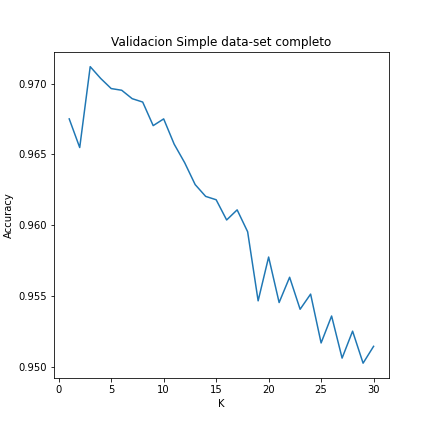
\includegraphics[width=8cm]{images/validacionSimple_datasetCompleto.png}%
    \qquad
    \caption{Validación Simple de kNN sobre el dataset completo}
    \label{knn_valSimple}%
\end{figure}

\begin{table}[h!]
    \begin{center}
        \begin{tabular}{|c|c|}
        \hline
        \textbf{$k$} & \textbf{accuracy} \\
        \hline
        3 &  0.9711\\
        4 & 0.9703\\
        5 & 0.9696\\
        6 & 0.9695\\
        7 &  0.9689\\
        8 & 0.9686\\
        1 & 0.9675\\
        10 & 0.9675\\
        9 & 0.9670\\
        11 & 0.9657\\
        
        \hline
        \end{tabular}
        \caption{Accuracy de las mejores 10 parejas extraido de la Validación Simple sobre el dataset completo para kNN.}
        \label{knn_valSimple_table}
    \end{center}
\end{table}

\subsubsection{kNN+PCA}

\par

$ k \in \{1,..,80\}$ (granularidad = 2)\\$alpha \in \{  35, 160 \}$ (granularidad = 5)

\begin{figure}[H]
    \centering
    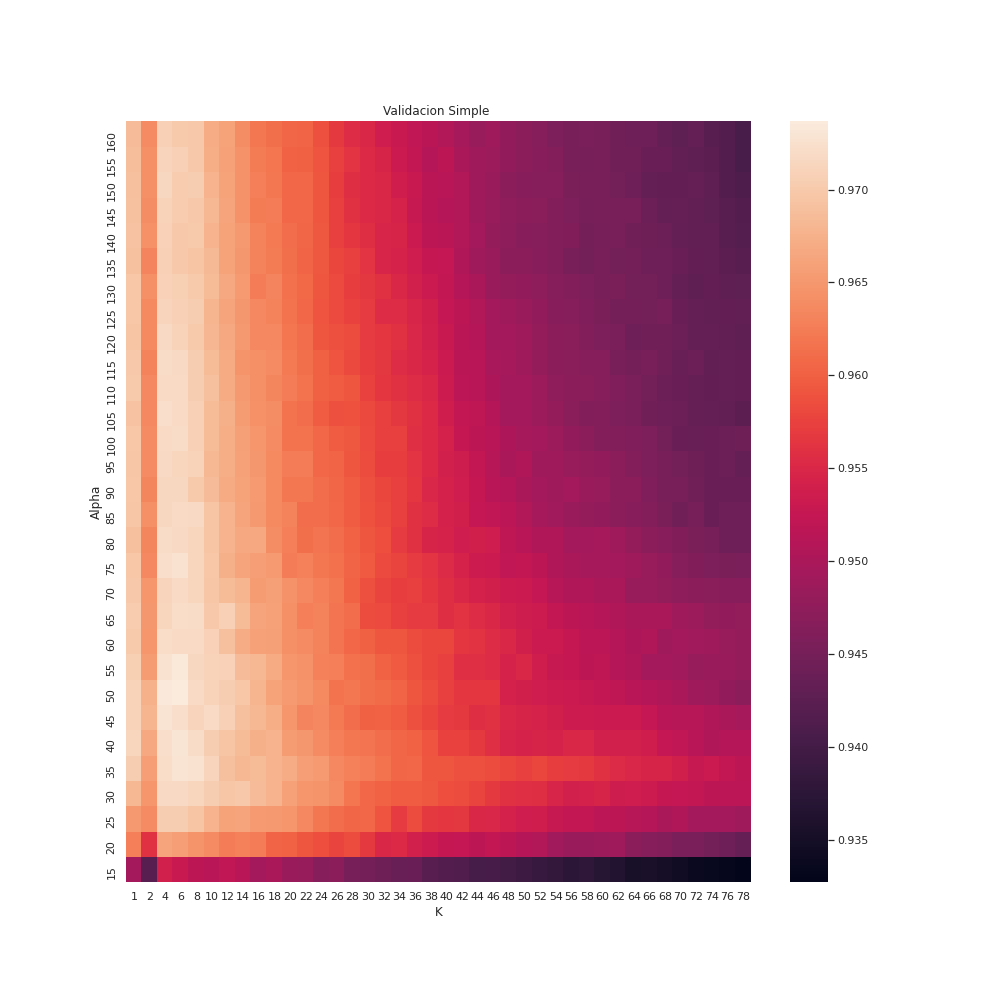
\includegraphics[width=12cm]{images/validacionSimple_datasetCompleto_knnpca_k80}%
    \qquad
    \caption{Validación Simple de kNN+PCA sobre el dataset completo}
    \label{knnpca_valSimpleCompleto}%
\end{figure}


\begin{table}[h!]
    \begin{center}
        \begin{tabular}{|c|c|c|c|}
        \hline
        \textbf{$k$} & \textbf{$\alpha$} & \textbf{accuracy} \\
        \hline
        50 & 6 & 0.9736\\
        50 & 4 & 0.9734\\
        55 & 6 & 0.9733\\
        40 & 6 & 0.9739\\
        35 & 6 & 0.9728\\
        45 & 4 & 0.9728\\
        35 & 8 & 0.9726\\
        75 & 6 & 0.9726\\
        55 & 4 & 0.9726\\
        45 & 6 & 0.9723\\
        
        \hline
        \end{tabular}
        \caption{Accuracy de las mejores 10 parejas extraído de la Validación Simple sobre el dataset completo para kNN+PCA.}
        \label{knnpca_valSimple_table}
    \end{center}
\end{table}

\subsection{Validación Cruzada}

Por último para conseguir el mejor parámetro o la mejor pareja en el caso de knn+pca se somete a los resultados previos a una corrida de validación cruzada ,con diez particiones, para evitar cualquier tipo de sesgo que pudiera tener nuestro anterior split de entrenamiento y validación. 
El funcionamiento de la validación cruzada junto a la elección de su parámetros como diez se detalla en la sección @LUIS.

\subsubsection{kNN}


$ k \in \{1,3,4,5,6,7,8,9,10,11\}$

\begin{table}[h!]
    \begin{center}
        \begin{tabular}{|c|c|}
        \hline
        \textbf{$k$} & \textbf{accuracy} \\
        \hline
        3 &  0.9671\\
        5 & 0.9668\\
        4 & 0.9664\\
        6 & 0.9656\\
        1 &  0.9654\\
        7 & 0.9653\\
        8 & 0.9640\\
        9 & 0.9633\\
        10 & 0.9629\\
        11 & 0.9623\\
        
        \hline
        \end{tabular}
        \caption{Accuracy promedio resultante de la Validación Cruzada para kNN.}
        \label{knn_crossVal_table}
    \end{center}
\end{table}

\subsubsection{kNN+PCA}

En el caso de kNN+PCA  no solo tomamos las diez mejores parejas resultantes de la validación simple si no que extraemos los alpha, k de ellas y sometemos a validación cruzada a la combinación de todos ellos parámetros.

$ k \in \{4,6,8\}$
\par
$alpha \in \{  35, 40, 45, 50, 55, 75 \}$
\begin{table}[h!]
    \begin{center}
        \begin{tabular}{|c|c|c|c|}
        \hline
        \textbf{$k$} & \textbf{$\alpha$} & \textbf{accuracy} \\
        \hline
        40 & 4 & 0.9716\\
        35 & 6 & 0.9713\\
        40 & 6 & 0.9712\\
        35 & 4 & 0.9712\\
        45 & 6 & 0.9711\\
        45 & 4 & 0.9711\\
        50 & 4 & 0.9710\\
        40 & 8 & 0.9710\\
        35 & 8 & 0.9710\\
        55 & 6 & 0.9708\\
        
        \hline
        \end{tabular}
        \caption{Accuracy de las mejores 10 parejas del total de 18 parejas extraído de la Validación Cruzada .}
        \label{knnpca_crossVal_table}

    \end{center}
\end{table}

\subsection{ Testing sobre la mejor pareja : }


Utilizamos el 20$\%$ del dataset previamente separado para testear conseguir el $Accuracy$ de la mejor pareja.

\subsubsection{kNN}

$Accuracy_{mejor pareja} = 0.9661 $
\par
\vspace{0.5cm}
Aclaración : la matriz de confusión se le reemplazaron los elementos de su diagonal por ceros para que sea más sencillo visualizar las demás casillas.
\begin{figure}[H]
    \centering
    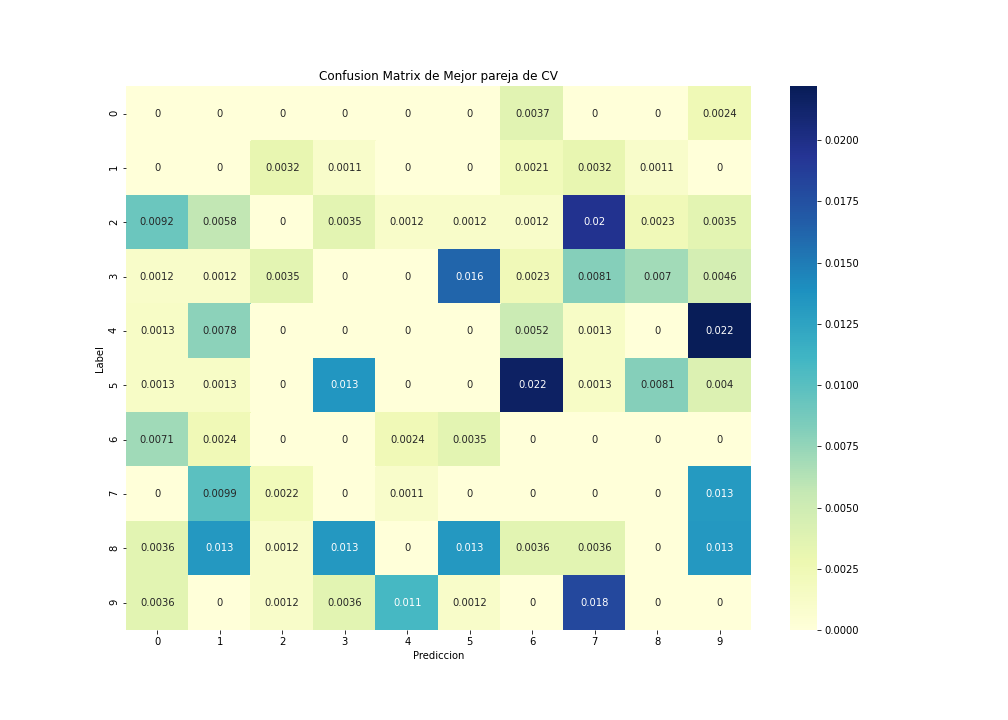
\includegraphics[width=14cm]{images/ConfMatrix_knn.png}%
    \qquad
    \caption{Matriz de Confusión para el mejor parámetro de kNN }
    \label{knn_MatrizConf}%
\end{figure}



\begin{figure}[H]
\begin{subfigure}{0.5\textwidth}
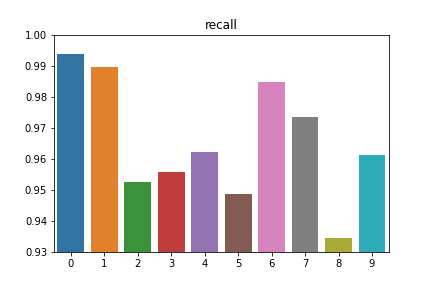
\includegraphics[width=0.9\linewidth, height=5cm]{images/recall_knn.png} 
\caption{Recall del mejor parámetro}
\end{subfigure}
\begin{subfigure}{0.5\textwidth}
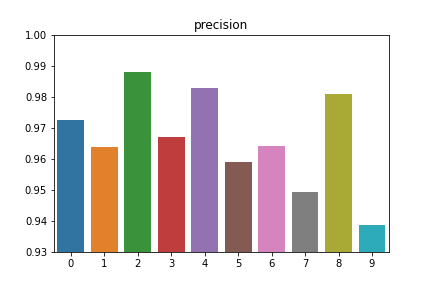
\includegraphics[width=0.9\linewidth, height=5cm]{images/precision_knn.png} 
\caption{Precision del mejor parámetro}
\end{subfigure}
\caption{Metricas del mejor parametros para kNN.}
\label{knn_metricas}%
\end{figure}





\subsubsection{kNN+PCA}


\vspace{0.5cm}
$Accuracy_{mejor pareja} = 0.9725 $
\par
\vspace{0.5cm}
Aclaracion : la matriz de confusión se le reemplazaron los elementos de su diagonal por ceros para que sea más sencillo visualizar las demás casillas.
\begin{figure}[H]
    \centering
    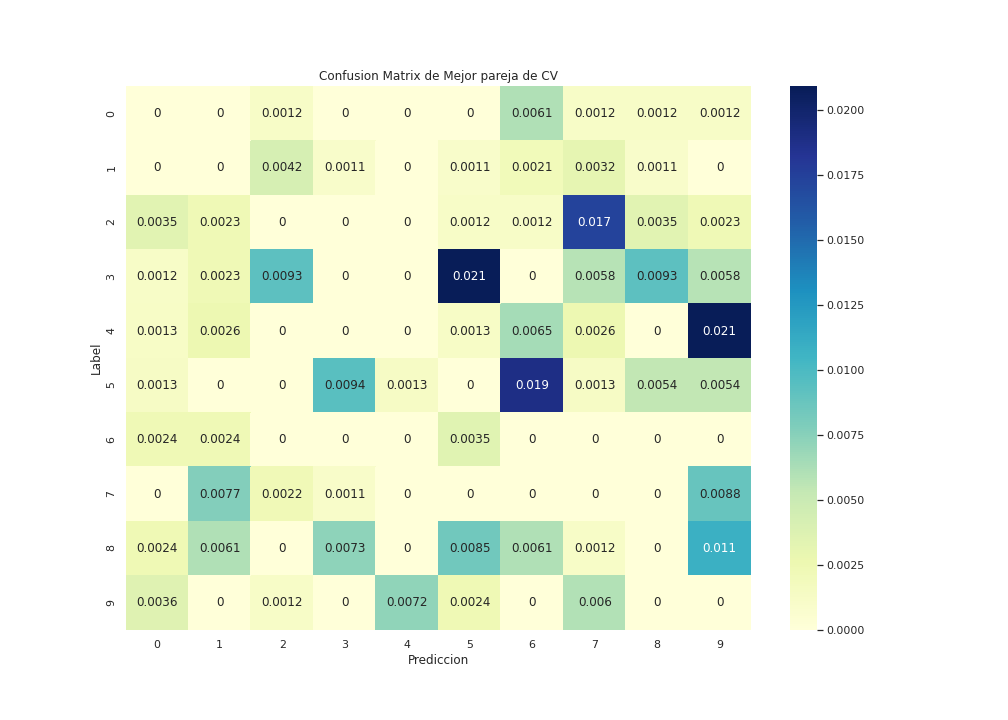
\includegraphics[width=14cm]{images/ConfMatrix_knnpca.png}%
    \qquad
    \caption{Matriz de Confusión para el mejor parámetro de kNN }
    \label{knnpca_MatrizConf}%
\end{figure}

\begin{figure}[h]
\begin{subfigure}{0.5\textwidth}
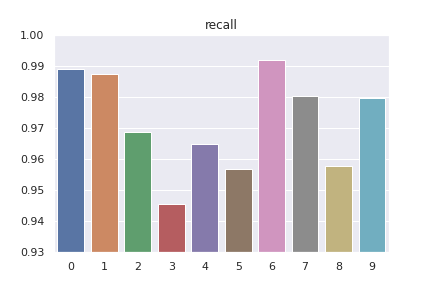
\includegraphics[width=0.9\linewidth, height=5cm]{images/recall_knnpca.png} 
\caption{Recall de la mejor pareja}
\label{fig:metpca1}
\end{subfigure}
\begin{subfigure}{0.5\textwidth}
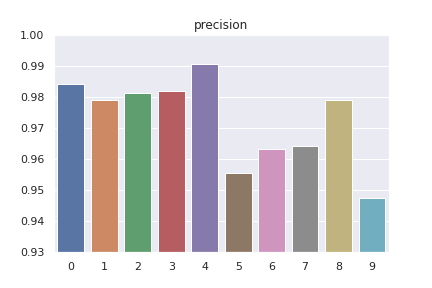
\includegraphics[width=0.9\linewidth, height=5cm]{images/precision_knnpca.png} 
\caption{Precision de la mejor pareja}
\label{fig:metpca2}
\end{subfigure}
\caption{Métricas de la mejor pareja para kNN+PCA.}
\label{knnpca_metricas}%
\end{figure}


\subsection{Conclusión de los parámetros óptimos}


Como se puede observar tanto en las métricas y matriz de confusión de kNN como kNN+PCA para algunos dígitos estos métodos funcionan casi perfectamente (es el caso del uno y el cero), pero para otros como el tres por ejemplo su rendimiento decrece. Estas disparidades en la predicción hacen que nos planteamos algunas dudas , si estos datos mal clasificados pueden considerarse como outliers dado a su morfología no se asemeja al dígito que dice su etiqueta o tal vez debemos modificar nuestro entrenamiento para llegar a mejorar la predicción de una clase complicado , si esto es así tal vez se deba dejar de lado el accuracy general.
%al vez el 
%como por ejemplo tal vez con alguna elección de  parámetros en las que baje un poco el accuracy general podríamos lograr un desempeño mejor en algunos de estos dígitos complicados, otra posibilidad sería que necesitamos más datos de esos dígitos para entrenar el método y así balancear el rendimiento de todas las clases.

